% Document layout
\documentclass[a4paper,11pt]{article}
\usepackage[a4paper, inner=2.5cm , outer=2.5cm, top=2cm, bottom=2cm]{geometry}
\usepackage[usenames,dvipsnames]{color}
% Referencing & fonts
\usepackage[sort&compress]{natbib}
\setlength{\bibsep}{0.0pt}
\usepackage[font=small,labelfont=bf]{caption}
\usepackage[OT2,T1]{fontenc}
% Set formats for each heading level
\usepackage{sectsty}
\allsectionsfont{\usefont{OT1}{phv}{bc}{n}\selectfont}
\sectionfont{\color{MidnightBlue}} % sets colour of sections
\subsectionfont{\color{MidnightBlue}}  % sets colour of subsections
\subsubsectionfont{\color{MidnightBlue}}  % sets colour of subsections
% Other shit
\usepackage{algorithm}
\usepackage{amsfonts}
\usepackage{amsmath}
\usepackage{amssymb}
\usepackage{bbm}
\usepackage{booktabs}
\usepackage{epsfig}
\usepackage{float}
\usepackage[font=normalsize]{caption}
\usepackage{graphicx}
\usepackage{hyperref}
\usepackage{lineno}
\usepackage{mathtools}
\usepackage{sidecap}
\usepackage{sectsty}
\usepackage{verbatim}
\usepackage{wrapfig}
\usepackage{xcolor}
% Declarations
\DeclarePairedDelimiter\floor{\lfloor}{\rfloor}
\DeclareSymbolFont{cyrletters}{OT2}{wncyr}{m}{n}
\DeclareMathSymbol{\Sha}{\mathalpha}{cyrletters}{"58}
\DeclareMathSymbol{\sha}{\mathalpha}{cyrletters}{"57}
% Defined commands
 \newcommand{\prgname}[1]{\textcolor{NavyBlue}{\texttt{#1}}}
 \newcommand{\linkfont}[1]{\textcolor{BurntOrange}{\textbf{#1}}}
\newcommand{\shellcmd}[1]{\\\indent\indent\texttt{\$ #1}}
\newcommand{\shellctd}[1]{\\\indent\indent\texttt{#1}}
\newcommand{\ra}[1]{\renewcommand{\arraystretch}{#1}}
\begin{document}
\begin{figure}
\centering
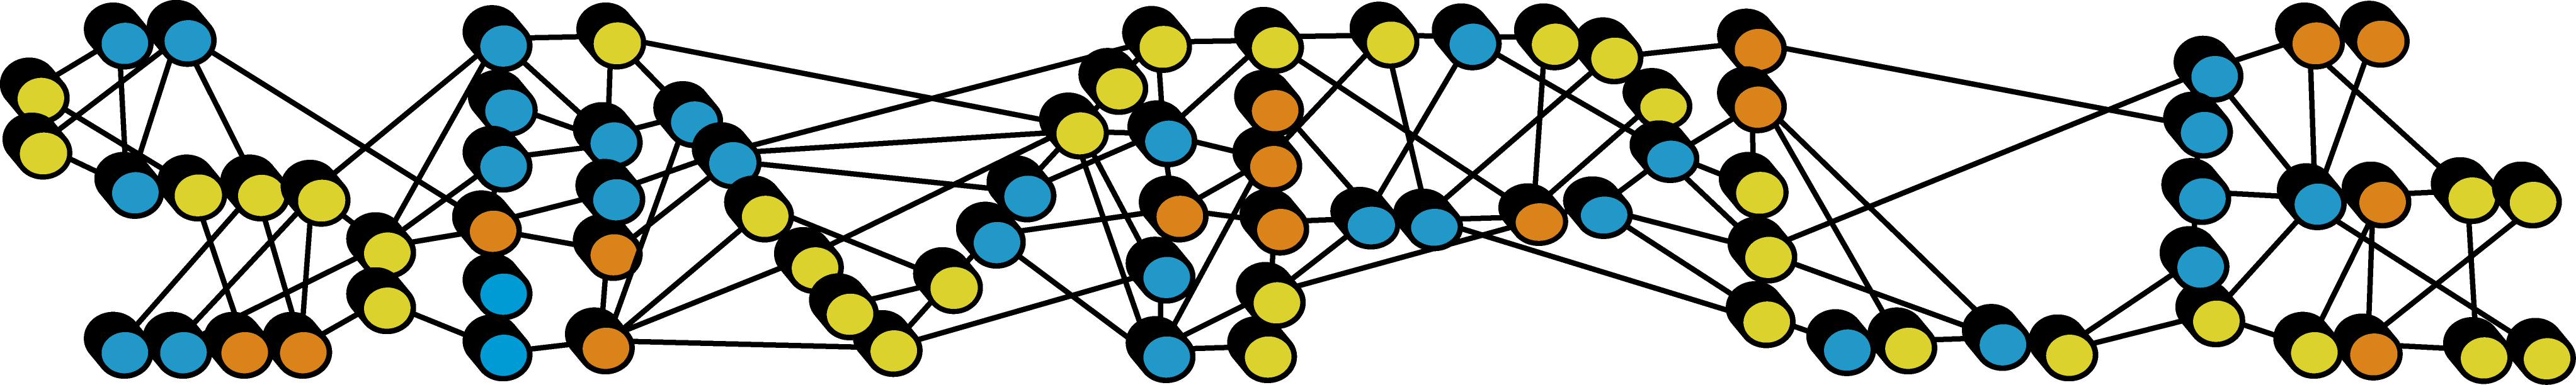
\includegraphics[keepaspectratio=true,scale=0.6]{../SIMPLE_logo/rawlogo}
%\caption{}
\end{figure}

\title{\prgname{The SIMPLE 3.0 Manual}}
\date{Jan 24, 2017}
\maketitle

\vspace{1em}
\begin{minipage}[ht]{0.48\textwidth}
\textbf{Contributors:}\\
cyril.reboul@monash.edu\\
michael.eager@monash.edu\\
dominika.elmlund@monash.edu\\
hans.elmlund@monash.edu\\
\textbf{Adress:}\\
Dept. Biochemistry and Molecular Biology\\
School of Biomedical Sciences\\
Monash University, Bldg. 77\\
Clayton, VIC, Australia, 3800\\
\textbf{Webpage:}\\
www.simplecryoem.com\\
\textbf{Contact:}\\
\url{http://simplecryoem.com/contact.html}\\
dominika@simplecryoem.com\\
\end{minipage}
\vspace{20pt}

\begin{quote}
\textbf{``Keep it SIMPLE stupid''}\\(\textit{Kelly Johnson}; lead engineer at the Lockheed Skunk Works, coined the famous KISS principle stating that systems work best if they are kept simple rather than made complex. Therefore, simplicity should be a key goal in design and unnecessary complexity should be avoided.)
\end{quote}

\begin{quote}
\textbf{``Everything should be made as SIMPLE as possible, but no SIMPLEr''}\\(\textit{Albert Einstein})
\end{quote}

\begin{quote}
\textbf{``Complex theories do not work, SIMPLE algorithms do''}\\(\textit{Vladimir N. Vapnik}; author of \textit{The Nature of Statistical Learning Theory})
\end{quote}
\clearpage

\tableofcontents{}
\clearpage

\section{About SIMPLE}

\textbf{S}ingle-particle \textbf{IM}age \textbf{P}rocessing \textbf{L}inux \textbf{E}ngine (\href{www.simplecryoem.com}{\textbf{\textcolor{BurntOrange}{SIMPLE}}}) is a program package for cryo-EM image processing, focusing on \textit{ab initio} 3D reconstruction of single-particles with any point-group symmetry. The SIMPLE back-end consists of an object-oriented numerical library written in modern Fortran. The SIMPLE front-end consists of many standalone, interoperable components developed according to the ``Unix toolkit philosophy''.

SIMPLE is free software: you can redistribute it and/or modify it under the terms of the \href{http://www.gnu.org/copyleft/gpl.html}{\textbf{\textcolor{BurntOrange}{GNU General Public License}}} as published by the Free Software Foundation, either version 3 of the license, or (at your option) any later version. SIMPLE is distributed with the hope that it will be useful, but WITHOUT ANY WARRANTY; without even the implied warranty of MERCHANTABILITY or FITNESS FOR A PARTICULAR PURPOSE. See the \href{http://www.gnu.org/copyleft/gpl.html}{\textbf{\textcolor{BurntOrange}{GNU General Public License}}} for more details.

\subsection{What is new in SIMPLE release 3.0?}
\begin{itemize}
    \item[--] 
    \item[--]
    \item[--]
\end{itemize}

\section{File Formats}

\subsection{Image File Formats}
SIMPLE supports SPIDER (\texttt{*.spi}) and MRC (\texttt{*.mrc}) formats for image stacks and volumes. The MRC file handling classes are shared with the the FREALIX program for helical reconstruction \citep{Rohou:2014aa}. RELION \citep{Scheres:2012aa} uses the convention that MRC stacks have the suffix \texttt{*.mrcs} and volumes the suffix \texttt{*.mrc}. This is to overcome the annoyance that it is not possible to tell from an MRC file header whether a MRC file is a volume or a stack. With SIMPLE you can select to use either the \texttt{*.mrcs} or \texttt{*.mrc} suffix for stacks. The way that we keep track of whether a file is a volume or stack is via the command line key value. The key-value pairs \texttt{vol1=rec.mrc} and \texttt{vol2=rec2.mrc} refer to volumes whereas the key-value pairs \texttt{stk=ptcls.mrc} and \texttt{stk2=ptcls2.mrc} refer to stacks.

\subsection{SIMPLE Parameter File Format}
The SIMPLE text-files used for parameter input/output use a \texttt{key=value} syntax of the form
\begin{verbatim}
e1=80. e2=100. e3=5.5 x=1.23 y=4.25 dfx=2.56 dfy=2.54 angast=30.5 state=1
\end{verbatim}
to represent per-particle information. Internally, the orientation information is stored in a dynamic hash data structure, which gives the file format high flexibility. Therefore, writing conversion scripts to allow interchange of parameters between SIMPLE and other packages is easy. SIMPLE uses the same conventions as FREALIGN \citep{Grigorieff:2007aa} to represent orientations and CTF parameters. The CTF parameterisation obtained by CTFFIND \citep{Mindell:2003aa} can be directly plugged into SIMPLE, for example by creating a file \texttt{deftab.txt}, looking like
\begin{verbatim}
kv=300 cs=2.7 fraca=0.07 dfx=2.56 dfy=2.76 angast=30.5
kv=300 cs=2.7 fraca=0.07 dfx=3.50 dfy=3.33 angast=60.0
kv=300 cs=2.7 fraca=0.07 dfx=1.98 dfy=2.02 angast=120.5
...
\end{verbatim}
and adding \texttt{deftab=deftab.txt} and \texttt{ctf=yes} to the PRIME command line (if the images are phase-flipped, this should be indicated by \texttt{ctf=flip}). Note that we now include \texttt{kv}, \texttt{cs}, and \texttt{fraca} in the document listing the CTF parameters. Having all the CTF parameters listed per particle allows easy merging of data sets from different microscopes. SIMPLE now implements a wrapper program for CTFFIND version 4.1.X and newer, producing a SIMPLE conforming document by executing CTFFIND in parallel (via \texttt{simple\_distr\_exec prg=ctffind}). If you have obtained CTF parameters with CTFFIND by other means (via RELION, for example) you can provide a plain text file with the two defocus values and the angle of astigmatism to the SIMPLE program \prgname{makedeftab} and it will take care of the formatting and unit conversions for you.

\subsection{Parameter File Conversions}
The \texttt{SIMPLE/scripts} folder contains a perl-script (\texttt{convert\_frealign2simple.pl}) to convert a Frealing parameter file to a SIMPLE parameter file. This is easy, since both software internally use the \href{http://spider.wadsworth.org/spider_doc/spider/docs/euler.html}{\textbf{\textcolor{BurntOrange}{Spider Euler angle convention}}}. Other packages may use other conventions. There's also a \texttt{convert\_relion2simple.pl} for extracting CTF parameters from RELION \texttt{*.star} files and a \texttt{relion2emanbox.pl} script for converting box files obtained with RELION to the EMAN \texttt{*.box} format used by SIMPLE.

\section{Installation Instructions}

\subsection{System requirements}
\begin{itemize}
	\item[--] Linux (we use Ubuntu 15.04 and above)
	\item[--] MacOSX: 10.10 and above
	\item[--] CMake 3.2 and above
	\item[--] FFTW 3.3 and above
	\item[--] GNU toolchain (gcc \& gfortran) 4.9 to 5.4
\end{itemize}

\subsection{Installation}
\noindent{}\textbf{Step 1:} Create the directory in which you are going to install SIMPLE (referred to here as \texttt{<simple\_path>})

\begin{verbatim}
        @!#> mkdir <simple_path>
\end{verbatim}

\noindent{}\textbf{Step 2:} Unzip the SIMPLE 3.0 tar ball in this directory (assuming you have downloaded the tar ball in the \texttt{<downloads>} directory)

\begin{verbatim}
        @!#> mv <downloads>/SIMPLE3.0.tgz <simple path>
        @!#> cd <simple path>
        @!#> tar -xzf SIMPLE3.0.tgz
\end{verbatim}

\noindent{}\textbf{Step 3:} Create a directory for the build

\begin{verbatim}
        @!#> cd simple3.0
        @!#> mkdir build
        @!#> cd build
\end{verbatim}

\noindent{}\textbf{Step 4:} Compile and install SIMPLE 3.0

\begin{verbatim}
        @!#> cmake ../
        @!#> make -j install
\end{verbatim}

\noindent{}This will install SIMPLE in the \texttt{'build'} directory. If you wish to provide an alternative installation directory, substitute step 4 with

\begin{verbatim}
        @!#> cmake -DCMAKE_INSTALL_PREFIX=<alternative directory> ../
        @!#> make -j install
\end{verbatim}

\noindent{}Step 4 assumes that gcc/gfortran and FFTW are installed in fairly standard directories on your machine. In case you have a 
more exotic setup you can provide the paths pointing to your custom gcc/gfortran \& FFTW by substituting step 4 with

\begin{verbatim}
        @!#> FC=<gcc/gfortran path> FFTW_DIR=<FFTW path> cmake ../
        @!#> make -j install
\end{verbatim}

\noindent{}For instance, on MacOS:
\begin{itemize}
	\item[--] Macports users may use: FC=/opt/local/bin/gfortran FFTW\_DIR=/opt/local;
	\item[--] Fink users: FC=/sw/bin/gfortran FFTW\_DIR=/sw/; and
	\item[--] Homebrew users: FC=/usr/local/bin/gfortran FFTW\_DIR=/usr/local/
\end{itemize}

\noindent{}\textbf{Step 5:} To run SIMPLE, the bin and scripts paths need to be in the \texttt{PATH} environment
variable and the lib path in the \texttt{LD\_LIBRARY\_PATH} variable. The \texttt{SIMPLE\_PATH} environment
 variable must also be defined. The shell scripts \texttt{add2.bashrc} and \texttt{add2.tcshrc} containing the necessary 
 instructions were generated during the build step. For immediate use for running and testing, execute
\begin{verbatim}
    @!#> source add2.bashrc
\end{verbatim}
\noindent{}or, for TCSH/CSH users:
\begin{verbatim}
    @!#> source add2.tcshrc
\end{verbatim}

\noindent{}For permanent installation \texttt{BASH} users should add the contents of \texttt{add2.bashrc} to your \texttt{<HOME>/.bashrc}
\begin{verbatim}
    @!#> cat add2.bashrc >> ~/.bashrc
\end{verbatim}
\noindent{}or for TCSH/CSH users:
\begin{verbatim}
    @!#> cat add2.tcshrc >> ~/.tcshrc
\end{verbatim}
\noindent{}To test the build, please execute
\begin{verbatim}
    @!#> make test
    @!#> ctest --output-on-failure
\end{verbatim}

\subsection{Testing the Most Important Features}

\noindent{}To ensure that SIMPLE has been correctly installed, we recommend running the application \texttt{simple\_test\_install}. It will test the most 
important components in the SIMPLE library  (those used by prime2D and  prime3D). Execute

\begin{verbatim}
        @!#> simple_test_install 
\end{verbatim}

\noindent{}The program will create its own folder \texttt{SIMPLE\_TEST\_INSTALL*date*} where temporary files and information about each 
test are stored. Upon succesful completion you should see

\begin{verbatim}
        @!#> **** SIMPLE_TEST_INSTALL NORMAL STOP ****
\end{verbatim}

\noindent{}\texttt{simple\_test\_install} can be executed anywhere. After execution, the folder created can be safely removed. If any of the individual 
tests fail an error message will be displayed. If you detect an error, please carefully check the SIMPLE and FFTW installations 
and the gfortran version. If you still have issues, please file a help ticket on the webpage.

\subsection{Installation/Configuration on a Linux Cluster}

Installation on a Linux cluster is essentially the same as on a Linux workstation with the exception that the appropriate modules need to be loaded before installation and execution. On a typical SLURM cluster
\begin{verbatim}
        @!#> module load fftw/3.3.4-gcc
        @!#> module load gcc/4.9.1
\end{verbatim}
The instructions for how to execute SIMPLE in distributed environments (clusters or workstations with more than one CPU socket) are described below \label{distr}.

\section{SIMPLE Usage}

\subsection{SIMPLE Help Tools}
In attempt to reduce the dependency on the manual, we have packaged a lot of the documentation in the software itself. For example
\begin{verbatim}
@!#> simple_exec prg=list
automask2D
automask3D
binarise
boxconvs
cavgassemble
cenvol
check2D_conv
check3D_conv
...
\end{verbatim}
lists all programs executed with \texttt{simple\_exec} (shared-memory parallelisation) and
\begin{verbatim}
@!#> simple_distr_exec prg=list
comlin_smat
ctffind
ini3D_from_cavgs
makecavgs
prime2D
prime3D
prime3D_init
recvol
symsrch
tseries_track
unblur
unblur_ctffind
unblur_tomo
\end{verbatim}
lists all distributed workflows executed with \texttt{simple\_distr\_exec}. If you don't quite remember which program you are looking for but remember that it was called \texttt{prime} something, you could execute
\begin{verbatim}
@!#> simple_distr_exec prg=list | grep prime
prime2D
prime3D
prime3D_init
\end{verbatim}
If you want a description for a particular program, for example \prgname{prime2D}, execute
\begin{verbatim}
@!#> simple_distr_exec prg=prime2D describe=yes
is a reference-free 2D alignment/clustering algorithm adopted from the 
prime3D probabilistic ab initio 3D reconstruction algorithm
\end{verbatim}
To obtain a description of the what command line options are available, execute
\begin{verbatim}
@!#> simple_distr_exec prg=prime2D
USAGE:
bash-3.2$ simple_distr_exec prg=simple_program key1=val1 key2=val2 ...

REQUIRED
stk  = particle stack with all images(ptcls.ext)
smpd = sampling distance, same as EMANs apix(in A)
msk  = mask radius(in pixels)
ncls = # clusters
ctf  = ctf flag(yes|no|flip)

OPTIONAL
nparts    = # partitions in distributed exection
chunksz   = # images/orientations in chunk
nthr      = # OpenMP threads{1}
ncunits   = # computing units, can be < nparts{nparts}
deftab    = text file with CTF info(*.txt/*.asc)
refs      = initial2Dreferences.ext
oritab    = table (text file) of orientations(*.asc/*.txt)
hp        = high-pass limit(in A)
lp        = low-pass limit(in A)
lpstart   = start low-pass limit(in A){15}
lpstop    = stop low-pass limit(in A){8}
cenlp     = low-pass limit for binarisation in centering(in A){30 A}
trs       = maximum halfwidth shift(in pixels)
automsk   = envelope masking(yes|no|cavg){no}
amsklp    = low-pass limit for envelope mask generation(in A)
inner     = inner mask radius(in pixels)
width     = falloff of inner mask(in pixels){10}
startit   = start iterating from here
maxits    = maximum # iterations
filwidth  = width of filament (in A)
center    = center image(s)/class average(s)/volume(s)(yes|no){no}
autoscale = automatic down-scaling(yes|no){yes}
oritab3D  = table (text file) of 3D orientations(*.asc/*.txt)
\end{verbatim}

\subsection{Execution of SIMPLE}
SIMPLE is executed primarily via \texttt{simple\_distr\_exec} that implements higher level workflows intended for distributed execution on workstations and clusters using a hybrid parallelisation model (distributed \textit{and} shared memory). SIMPLE can also be executed via \texttt{simple\_exec}, which implements all individual SIMPLE programs and runs in shared-memory parallelisation mode. Please, beware that the high-level workflows (\prgname{prime2D} and \prgname{ini3D\_from\_cavgs}, for example) can \textit{only} be executed via the distributed execution route. In cluster environments using a job scheduler (PBS, SLURM and SGE are supported by SIMPLE) the file \texttt{simple\_distr\_config.env} in the current working directory controls the execution.
\begin{verbatim}
bash-3.2$ cat simple_distr_config.env 
# CONFIGURATION FILE FOR DISTRIBUTED SIMPLE EXECUTION

# ABSOLUTE PATH TO SIMPLE ROOT DIRECTORY
simple_path           = /scratch/m3earlyadopters/simple/simple/

# ESTIMATED TIME PER IMAGE (IN SECONDS)
time_per_image        = 600

# USER DETAILS
user_account          = el85 
user_email            = hans.elmlund@monash.edu
user_project          = 

# QSYS DETAILS (qsys_name=<local|slurm|pbs>)
qsys_name             = slurm
qsys_partition        = m3a
qsys_qos              =
qsys_reservation      = simple

# JOB DETAILS
job_ntasks            = 1
job_memory_per_task   = 48000
job_name              = taf-dna-part2
job_ntasks_per_socket = 1
\end{verbatim}
This file is auto-generated on workstations, but it needs to be edited by the user in cluster environments. If you need help configuring distributed SIMPLE execution, please file a help ticket on the webpage. The two most important parameters for distributed execution is the number of partitions \texttt{nparts} and the number of shared-memory CPU threads \texttt{nthr}. A rule of thumb for good performance on multi-socket workstations is to minimise the number of parts and maximising the number of threads subject to never having fewer parts than sockets. The shared memory parallelisation does not benefit from the use of a larger number of threads than the number of logical threads available on a socket. To check the number of processors on a linux system, execute \texttt{nproc} in the terminal. Consider a heterogeneous cluster with N nodes, two CPU sockets per node and six CPUs per socket.
\begin{SCfigure}[][h]
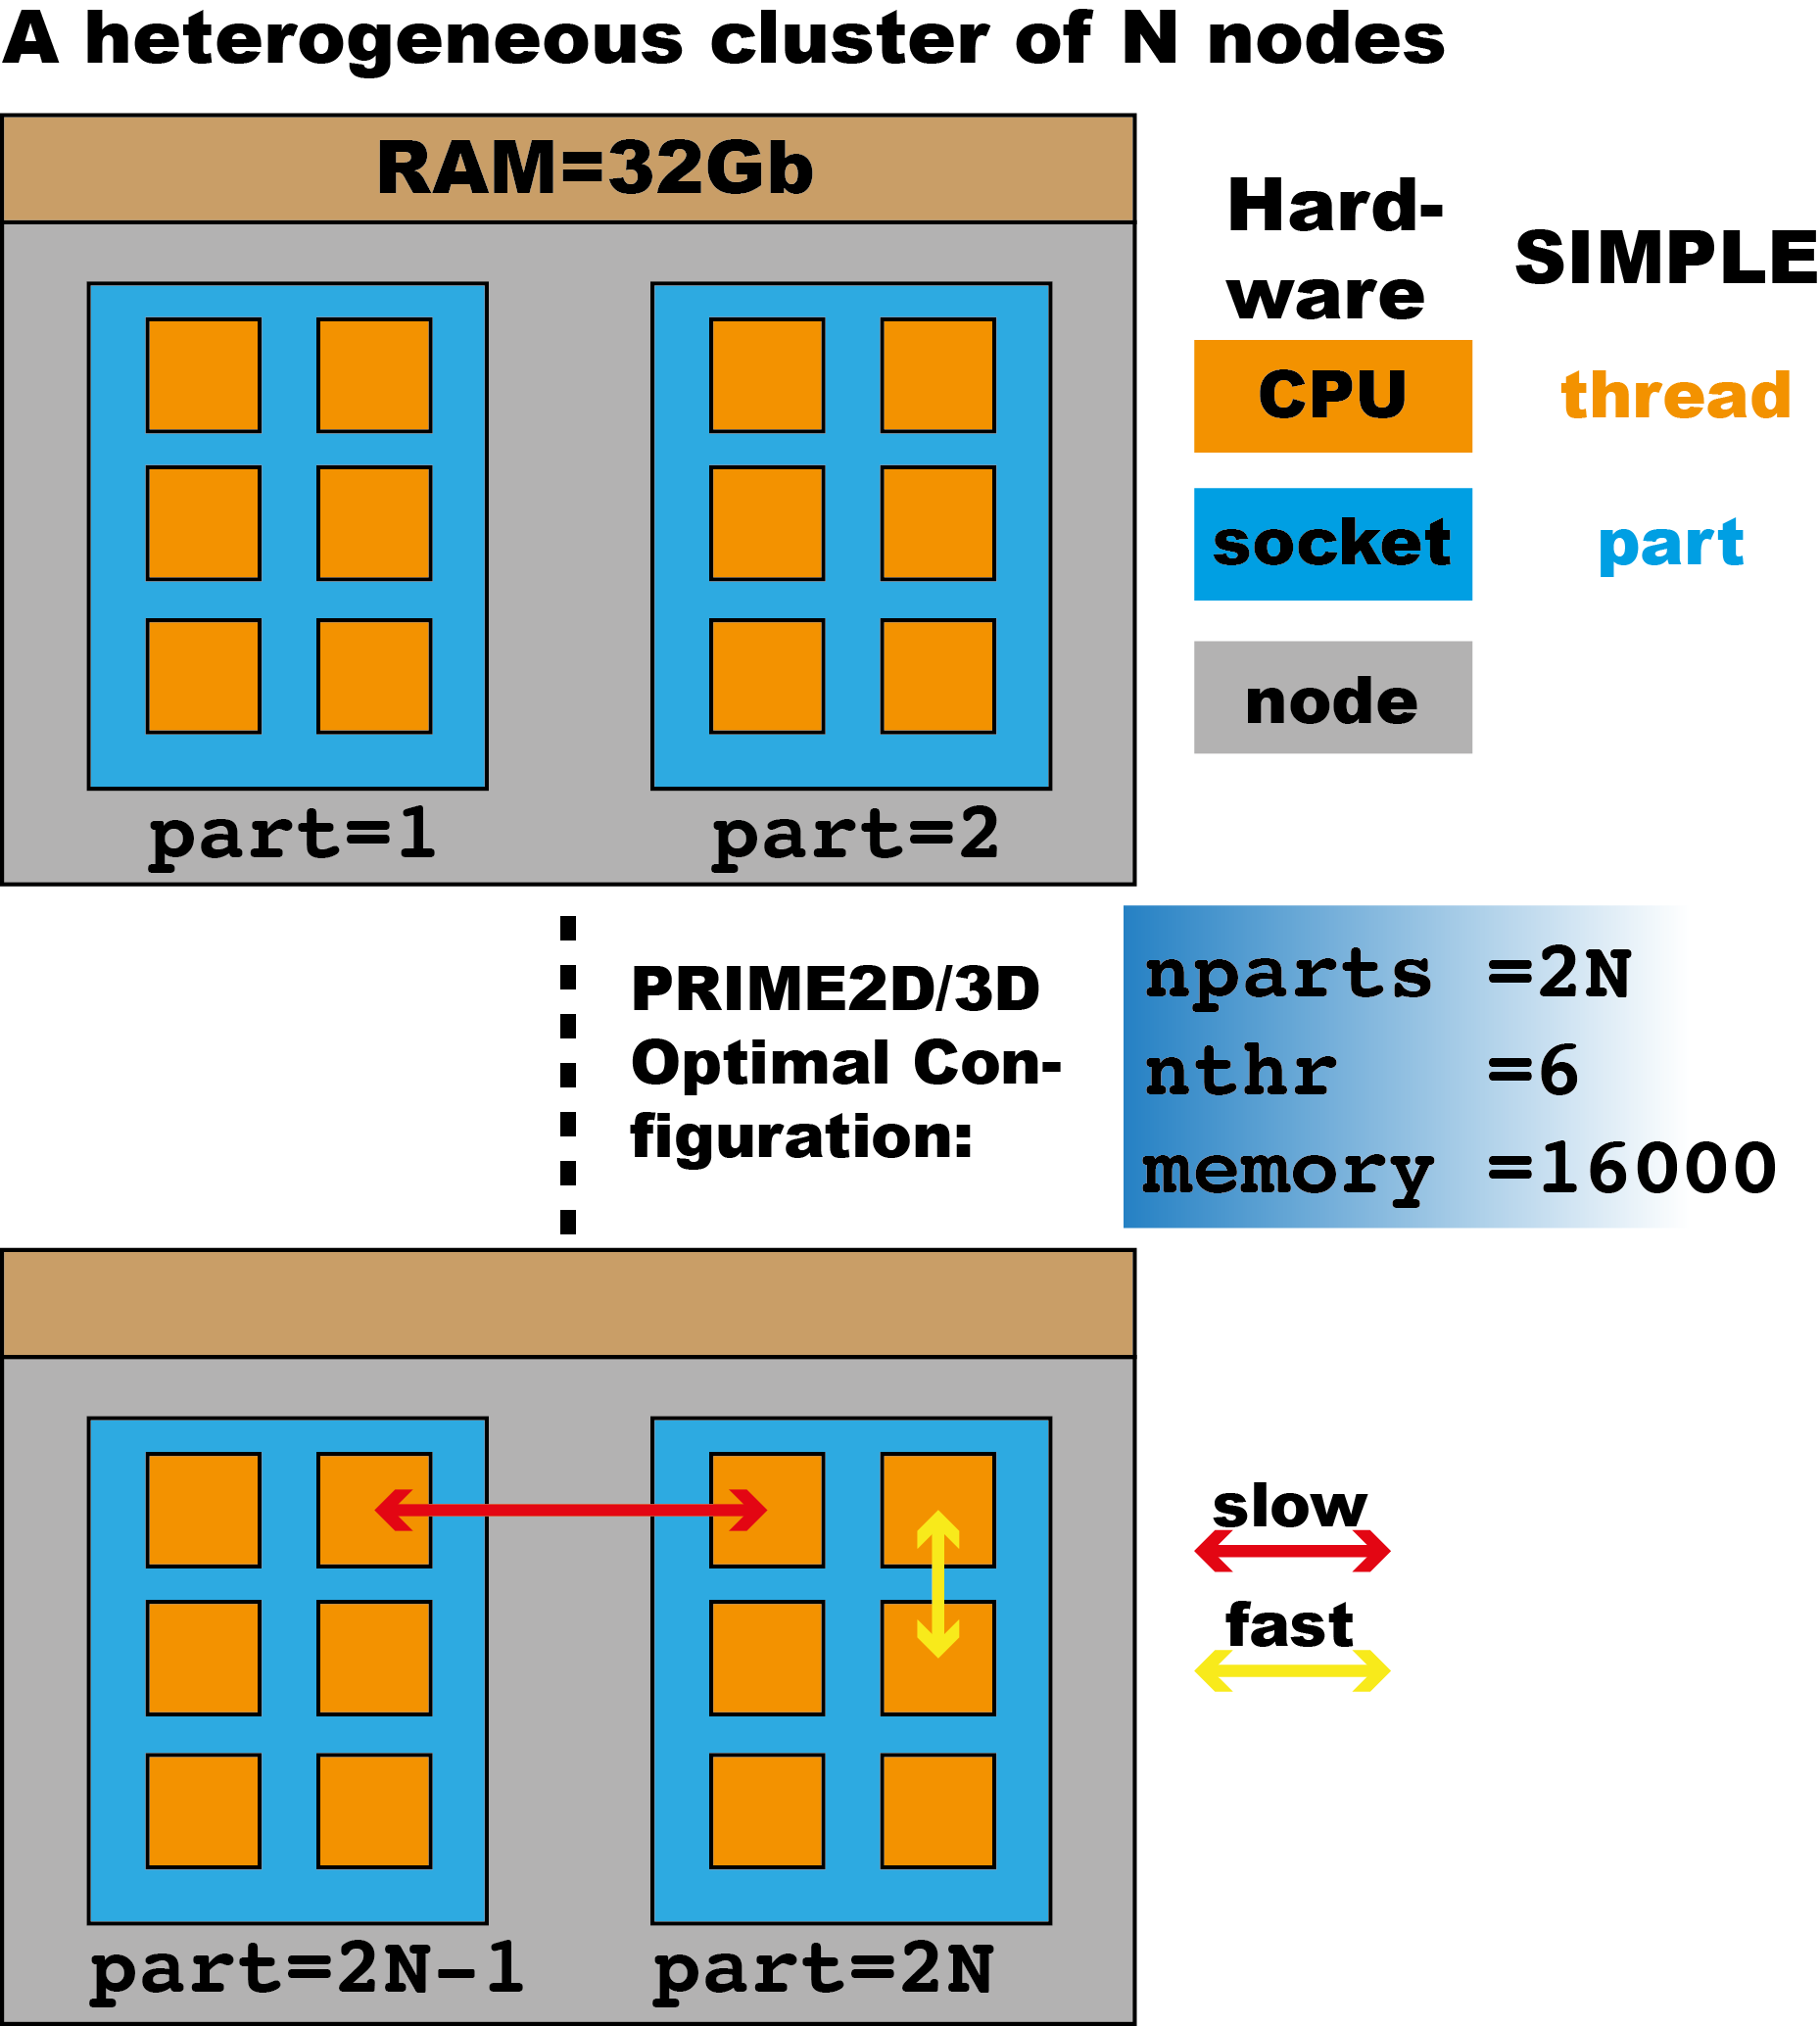
\includegraphics[keepaspectratio=true,scale=0.6]{../CPUtopo/cputopo}
\caption{\textbf{Configuration of the parallel PRIME-2D/3D execution on a heterogeneous cluster.} We here represent the nodes in  a heterogeneous cluster by two sockets with six CPUs each and 32Gb RAM/node. The best performance of PRIME--2D/3D is going to be obtained by partitioning  the jobs into \texttt{npart=2N} partitions, where \texttt{N} is the number of nodes. Each partition will then execute six threads \texttt{nthr=6} and these six threads will get access to half the RAM on the node (\texttt{memory=16000}) because we have two sockets per node that need to share the RAM between them}
\end{SCfigure}
If you are unsure how to configure your SIMPLE execution please file a help ticket.

We normally let \prgname{simple\_distr\_exec} run in the background on the login node of our cluster. An example of how to distribute \prgname{prime2D} using ten nodes is provided below.
\begin{verbatim}
@!#> nohup simple_distr_exec prg=prime2D stk=ptcls.mrc smpd=1.77 msk=100
ncls=600 nthr=8 nparts=10 >> PRIME2DOUT &
\end{verbatim}
Another option available on clusters that use the SLURM scheduler is to use the \texttt{srun} command for \prgname{simple\_distr\_exec} via
\begin{verbatim}
@!#> srun --ntasks=1 --ntasks-per-socket=1 --cpus-per-task=1 --mem=32000 
--time=2-0:0:0 --output=PRIME2DOUT.%j --error=PRIME2DERR.%j
simple_distr_exec prg=prime2D stk=ptcls.mrc smpd=1.77 msk=100
ncls=600 nthr=8 nparts=10 &
\end{verbatim}
However, beta testers have reported that srun job sometimes dies with no warning, possibly because of the low tolerance for network errors. A more robust route may be to use \texttt{sbatch} as follows
\begin{verbatim}
@!#>  sbatch -p MYCLUSTER --wrap="simple_distr_exec prg=prime2D stk=ptcls.mrc 
smpd=1.77 msk=100 ncls=600 nthr=8 nparts=10 >> PRIME2DOUT"
\end{verbatim}
where the \texttt{--wrap} flag automatically generates a bash script for the given command.

\subsection{From Movies to Near-atomic Resolution Map}
These steps describe a typical SIMPLE workflow.
\begin{enumerate}
\item DDD (Direct Detector Device) movie alignment and frame-weighting using SIMPLE program \prgname{unblur}, executed with \texttt{simple\_distr\_exec}
\item CTF parameter identification with the SIMPLE program \prgname{ctffind}, wrapping CTFFIND4 \citep{rohou2015ctffind4}, executed with \texttt{simple\_distr\_exec}
\item Particle identification using EMAN2 \citep{Tang:2007aa} to generate \texttt{*.box} files
\item Particle extraction with SIMPLE program \prgname{extract}, executed with \texttt{simple\_exec}
\item 2D analysis using the SIMPLE \prgname{prime2D} distributed workflow, executed with \texttt{simple\_distr\_exec}
\item \textit{Ab initio} 3D reconstruction from class averages using the SIMPLE \prgname{ini3D\_from\_cavgs} distributed workflow, executed with \texttt{simple\_distr\_exec}
\item Mapping of class average selection and 3D class orientations to the particles using SIMPLE program \prgname{map2ptcls}, executed with \texttt{simple\_exec}
\item Reconstruction of a 3D map from the individual particle images with SIMPLE program \prgname{recvol}, executed with \texttt{simple\_distr\_exec}
\item Map refinement will be part of release 3.0
\end{enumerate}
For descriptions for how to execute the individual steps, please refer to the documentation of each program (below).

\subsection{Workflows for Analysis of Time-series data of Nanoparticles Spinning in Solution}
In addition to providing algorithms for analysis of electron microscopic projection images of biological molecules, SIMPLE also provides support for time-series analysis of nanoparticles spinning in solution.
\subsubsection{Time-series Pre-processing}
\begin{enumerate}
\item Convert the time-series from \texttt{*.dm4} format to the \texttt{*.mrc} format using the \prgname{dm42mrc.pl} script. This script assumes that you have \texttt{EMAN2} installed on your system.
\item Use the \prgname{tseries\_extract} program to generate overlapping windows of frames in the time series. We recommend a window size of 5. This program is executed via \texttt{simple\_exec prg=tseries\_extract}. The \texttt{frameavg} flag controls the size of the time-window.
\item Correct for stage drift and global beam-induced motion by processing the \texttt{*tseries\_frames*} stacks with \prgname{unblur}. It is important that you set \texttt{lpstart=5} and \texttt{lpstop=3} in addition to the required input parameters.
\item Use \texttt{EMAN1.9} or \texttt{EMAN2} to identify, in the first motion corrected frame, the particles that you want to track throughout the time-series. Write out a \texttt{*.box} file with the particle coordinates.
\item Use the \texttt{*.box} file created in the previous step in conjunction with the motion-corrected frames as input to the program \prgname{tseries\_track} to generate individual stacks of images representing the windowed nanoparticles as a function of time from the first to the last frame. Please execute \prgname{tseries\_track} using the \texttt{simple\_distr\_exec} binary. This will run the tracker in parallel mode with one CPU allocated per particle. The \texttt{ncunit} parameter controls the number of CPUs being used and this number cannot be larger than the number of particles to track in parallel.
Once the pre-processing workflow has been finalised, the problem becomes a standard single-particle reconstruction problem (one per particle stack). However, as SIMPLE was originally designed for biological single-particle EM image processing, there are a few parameter tuning strategies to consider (described below).
\end{enumerate}

\def\bibfont{\footnotesize}
\bibliographystyle{cell}
\bibliography{Prime2bibfile}

\end{document}
